\newpage
\section{Extrahieren und transformieren der Daten[EK]}
\subsection{Producer in Python}
Der zur Phase-1 gehörige Producer ist ein in Python geschriebenes Programm, welches einen Grundstein für weitere Bemühungen in Phase-2 sein soll. Der Producer repräsentiert im theoretischen Model den Extrakt und die Transformation. 
\subsubsection{Kafka-Producer}
Die namensgebende Kafka-Library sorgt dafür, dass eine Verbindung mit dem Kafka-Broker aufgebaut werden kann.
\begin{lstlisting}[caption={Producer-Code}]
class Producer(object):
    def __init__(self, brokers):
        self.__producer = KafkaProducer(
            value_serializer=lambda v: json.dumps(v).encode('utf-8'),
            bootstrap_servers=brokers)

    def send_page_data(self, topic, key, data):
        key_bytes = bytes(key, encoding=‘utf-8')
        result = self.__producer.send(
            topic,
            key=key_bytes,
            value=data
        ).add_errback(on_error).add_callback(on_success)
\end{lstlisting}
\vspace{4mm}\par
\subsubsection{Init-Funktion}
Diese Funktion legt eine neue Instanz des Kafka-Producers an, um dies zu realisieren, muss eine Adresse des Brokers übergeben werden. Läuft eine Kafka-Instanz lokal würde als Beispiel die folgende Adresse der Funktion mitgeben werden: localhost:9092. Bei 9092 handelt es sich übrigens um den Standardport von Kafka.
\subsubsection{Send-Page-Data-Funktion}
Mithilfe dieser Funktion werden die Daten übermittelt. Mit dem Topic-Parameter wird der Namen des Topics mitgegeben mit, so können die Daten - in diesem Fall ein JSON-Objekt - eindeutig im Broker zugewiesen werden, danach muss der Load-Prozess sich nur noch auf dieses Topic abonnieren, um die gesendeten Daten zu erhalten. Liegt das angegebene Topic noch nicht im Broker vor, so wird dies automatisch erstellt.
\subsubsection{Parse-Log-Line}
Aus der folgenden Funktion kann entnommen werden, wie ein vereinfachter Extrakt-Prozess aussieht:
\begin{lstlisting}[caption={Extract-Code}]
def parse_log_line(line):
    strptime = datetime.datetime.strptime
    hostname = socket.gethostname()
    time = line.split(' ')[3][1::]
    entry = {}
    entry['timestamp'] = str(to_epoch(strptime(
        time, "%d/%b/%Y:%H:%M:%S")))
    entry['source'] = "{}".format(hostname)
    entry['type'] = "www_access"
    entry['log'] = "'{}'".format(line.rstrip())
    return entry
\end{lstlisting}
\vspace{4mm}\par
Über den Line-Parameter bekommt man die aktuelle eingelesene Zeile des Logfiles, welche zuvor durch den Fake-Apache-Log-Generator erstellt wurde. Die entnommen Daten werden dann mit Zeitstempel, Datentyp, Quelle und dem eigentlichen Log in einem Entry-Dictionary abgespeichert. 
\subsubsection{Show-Entry}
Das zuvor erstellte Entry-Dictionary  wird in der folgenden Funktion zu einem JSON-Object transformiert:
\begin{lstlisting}[caption={Tranform-Code}]
def show_entry(entry):
    temp = ",".join([
        entry['timestamp'],
        entry['source'],
        entry['type'],
        entry['log']
    ])
    log_entry = {'log': entry}
    temp = json.dumps(log_entry)
    logging.info("{}".format(temp))
    return temp
\end{lstlisting}
\vspace{4mm}\par
Nachdem das Entry zu einem JSON konvertiert wurde, erhält \textit{temp} den JSON-String, dieser wird vor der Rückgabe nochmals über das Log-File ausgegeben.
\subsubsection{Main}
In der Main-Funktion kommen alle zuvor genannten Funktionen zusammen und bilden so die Extraktion über die Transformation bis zum Weitersenden an Kafka: 
\begin{lstlisting}[caption={Main-Code}]
def main():
    kh = os.getenv('KH', 'localhost')
    kp = os.getenv('KP', '9092')
    ks = kh + ':' + str(kp)
    logging.info('Kafka server %s', ks)

    brokers = [ks]
    logging.info('KS: %s', str(brokers))
    logfile = open('/data/access.log')
    logfile.seek(0, 2)
    producer = Producer(brokers)
    while True:
        line = logfile.readline()
        if not line:
            time.sleep(0.1)
            continue
        else:
            entry = parse_log_line(line)
            if not entry:
                continue
            json_entry = show_entry(entry)
            producer.send_page_data('log', 'www_access', json_entry)
\end{lstlisting}
\vspace{4mm}\par
Anfangs werden die Defaultwerte gesetzt, welche der lokalen Standardkonfiguration von Kafka entsprechen, falls die Umgebungsvariabeln nicht vorhanden sind. Hier findet auch der Leseprozess der vom Generator generierten access.log statt. Dieses Log-File wird dann Zeile für Zeile zur Weiterverarbeitung an die für die Extraktion zuständige Funktion übergeben.
\newpage
\subsection{Kommunikation über Kafka}
\subsubsection{Einrichtung}
Mithilfe von Kafka erfolgt die Kommunikation zwischen dem ET-Prozess und des Load-Prozess über ein gemeinsames Topic. Der Kafka-Server läuft über eine eigene EC2-Maschine und wird dort mit Minimalkonfiguration ausgeführt. Als Referenz für diese Konfiguration diente die offizielle Apache Kafka Website. (vgl. \cite{Kafka-Quickstart})
\vspace{4mm}\par
Um die Kommunikation mit den anderen EC2-Machinen zu ermöglichen, muss zuerst die entsprechende Security-Group-Rule wie folgt im Bild gezeigt, in AWS vorgenommen werden.
\begin{figure}[H]
    \centering
    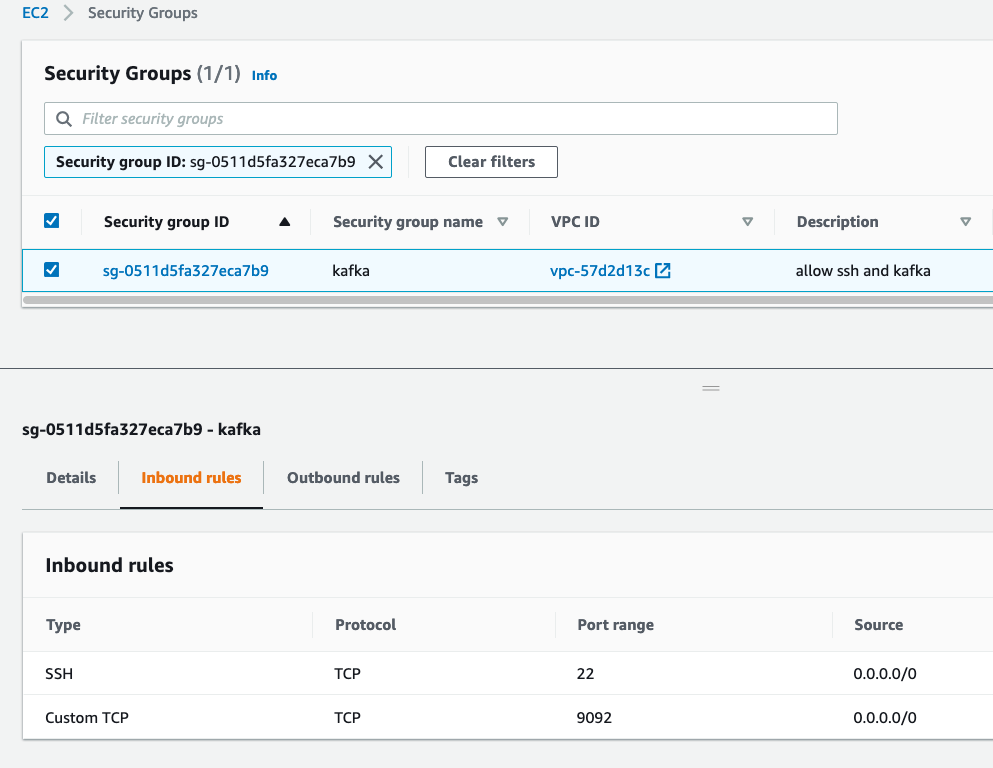
\includegraphics[scale=0.35]{images/aws-kafka-security.png}
    \caption{AWS-Security-Group (02.04.2020)}
\end{figure}
\newpage
Vor dem Start des Kafka-Servers muss Zookeeper gestartet werden: 
(Die Gründe dafür werden bei 4.2.2 und 4.2.3 in den Technologien erläutert)
\begin{lstlisting}[caption={Zookeeper-Start}]
> bin/zookeeper-server-start.sh config/zookeeper.properties
\end{lstlisting}
\vspace{4mm}\par
Läuft unser Zookeeper-Server kann nun der Kafka-Server über folgendes Kommando gestartet werden: 
\begin{lstlisting}[caption={Kafka-Start}]
> bin/kafka-server-start.sh config/server.properties
\end{lstlisting}
\vspace{4mm}\par
Um nun zu sehen, ob durch den \textit{Producer} ein Topic angelegt wurde, wird dies durch folgendes Kommando geprüft:
\begin{lstlisting}[caption={Topic-Check}]
> bin/kafka-topics.sh --list --bootstrap-server localhost:9092
> topicname
\end{lstlisting}
Anstatt \textit{topicname} sollte nun das Topic, unter welchem die Daten geschickt werden, sichtbar sein.
\subsubsection{Probleme und Lösungen}
Diese einfache Minimalkonfiguration wurde in Folge dessen aufgebaut, da die ursprüngliche Lösung keine Verbindung zu Stande bringen konnte. Erschwert wurde dies auch durch den komplexen Aufbau zweier separater Docker-Container
für Kafka und Zookeeper, welche wiederum auf der gleichen EC2-Maschine laufen sollten wie der Extrakt- und Transformationsprozess. Eine Verbindung innerhalb der Maschine konnte verwirklicht werden. Das Problem kam jedoch bei der Kommunikation mit der Load-Maschine auf. Daraufhin hatte die Firma die Entscheidung getroffen, dass Kafka und Zookeeper ohne Docker auf einer gemeinsamen separaten Maschine laufen sollten.
